\section{Appendix}

\subsection{Hernquist Models: Check of Integration routines}
To check the correct function of the integration routine, we used the
analytic formulas from \cite{Hernquist1990}:

\begin{eqnarray}
M(r) &=& M\frac{r^2}{(r+a)^2}\\
\nu(r) &=& \frac{M}{2\pi}\frac{a}{r}\frac{1}{(r+a)^3}\\
\beta(r) &=& 0
\end{eqnarray}

with mass scale $M$ and length scale $a$ as inputs, and calculated
$\siglos(r)$ with our numerical routine, including three
integrations. Working with extrapolations to the first bin turns out
to give the most stable results, corresponding nicely to the analytic
value \bcite{BaesDejonghe2002} of

\begin{eqnarray*}
\siglos(r) &=& \frac{1}{I(r)}\frac{1}{24\pi(1-r^2)^3}\times\\
           && \qquad [3r^2(20-35r^2+28r^4-8r^6)X(r) \\
           && \qquad + (6-65r^2+68r^4-24r^6)]-\frac{r}{2},\\
\sigma_r(r) &=& r(1+r)^3 \ln\left(\frac{1+r}{r}\right)\\
 &&\qquad-\frac{r(25+52r+42r^2+12r^3)}{12(1+r)},\\
I(r) &=& \frac{1}{2\pi}\frac{(2+r^2)X(r)-3}{(1-r^2)^2},\\
X(r) &=& \begin{cases}(1-r^2)^{-1/2} \text{arcsech}\,r,& \text{for}\,0\leq r\leq 1,\\
                (r^2-1)^{-1/2} \text{arcsecans}\,r,& \text{for}\,1\leq r\leq\infty
                \end{cases}.
\end{eqnarray*}



A single component model is set up according a simple Dehnen split
power-law sphere \cite{Read+2006},

\begin{equation}
  \rho(r) = \frac{M_\infty(3-\gamma)}{4\pi r_S}\left(\frac{r}{r_S}\right)^{-\gamma}\left(1+\frac{r}{r_S}\right)^{4-\gamma},
\end{equation}

where $M_\infty=1$ denotes the total mass, $\gamma=1$ the logarithmic
central asymptotic slope, and $r_S=1$ the scale length. We use $10^6$
sample points, outof which $10^4$ are extracted for further analysis.

We then let $\nu, \rho, \beta$ vary. The MCMC correctly recovers the
underlying mass distribution.



\subsection{Data quality}
How many tracer stars are needed to determine the overall density
profile reliably? To address this question, we performed three runs
with a restricted set of tracer particles. In the first, $10^3$
particles were chosen out of the $10^6$ simulated particles. With
$10^4$ particles, the confidence intervals shrink. These $10^4$
particles are split then into two populations of each $5\cdot10^3$
particles, with different scalelengths of $r_S$ and $r_S/10$. Most of
the second population particles are inside the first two bins, so the
overall convergence is not visibly affected above the third bin.
However, the models are better constrained around the scalelengths of
both tracer populations. This is expected from
\citet{WalkerPenarrubia2011}, as any velocity anisotropy sampling
yields the same mass constraint there.


\begin{figure*}
\begin{center}
\hspace{-7mm}
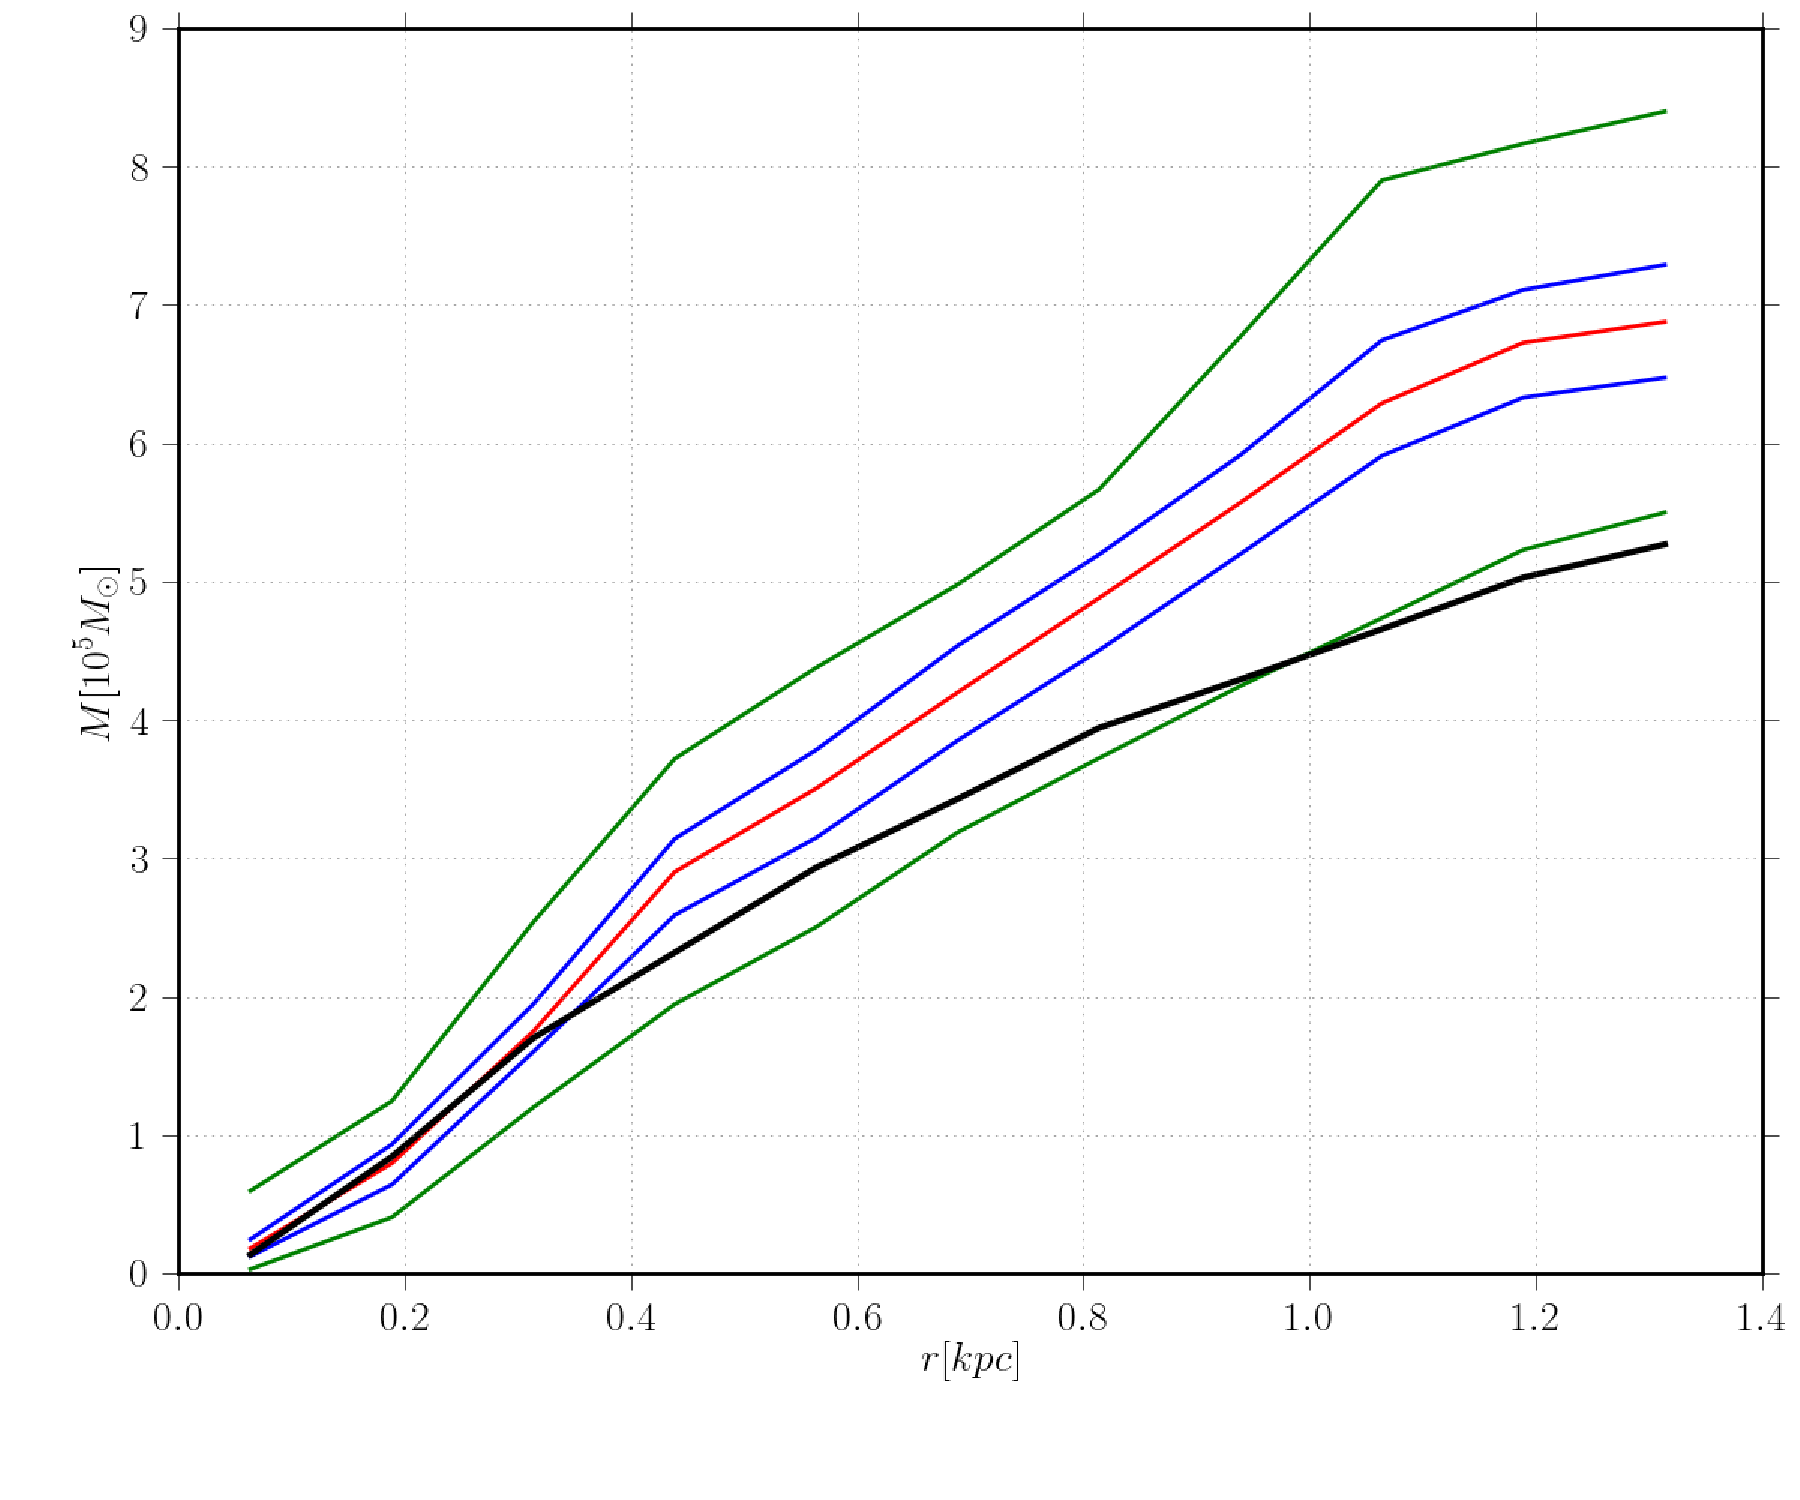
\includegraphics[width=0.3\textwidth]{fig/hernquist1e3.pdf}
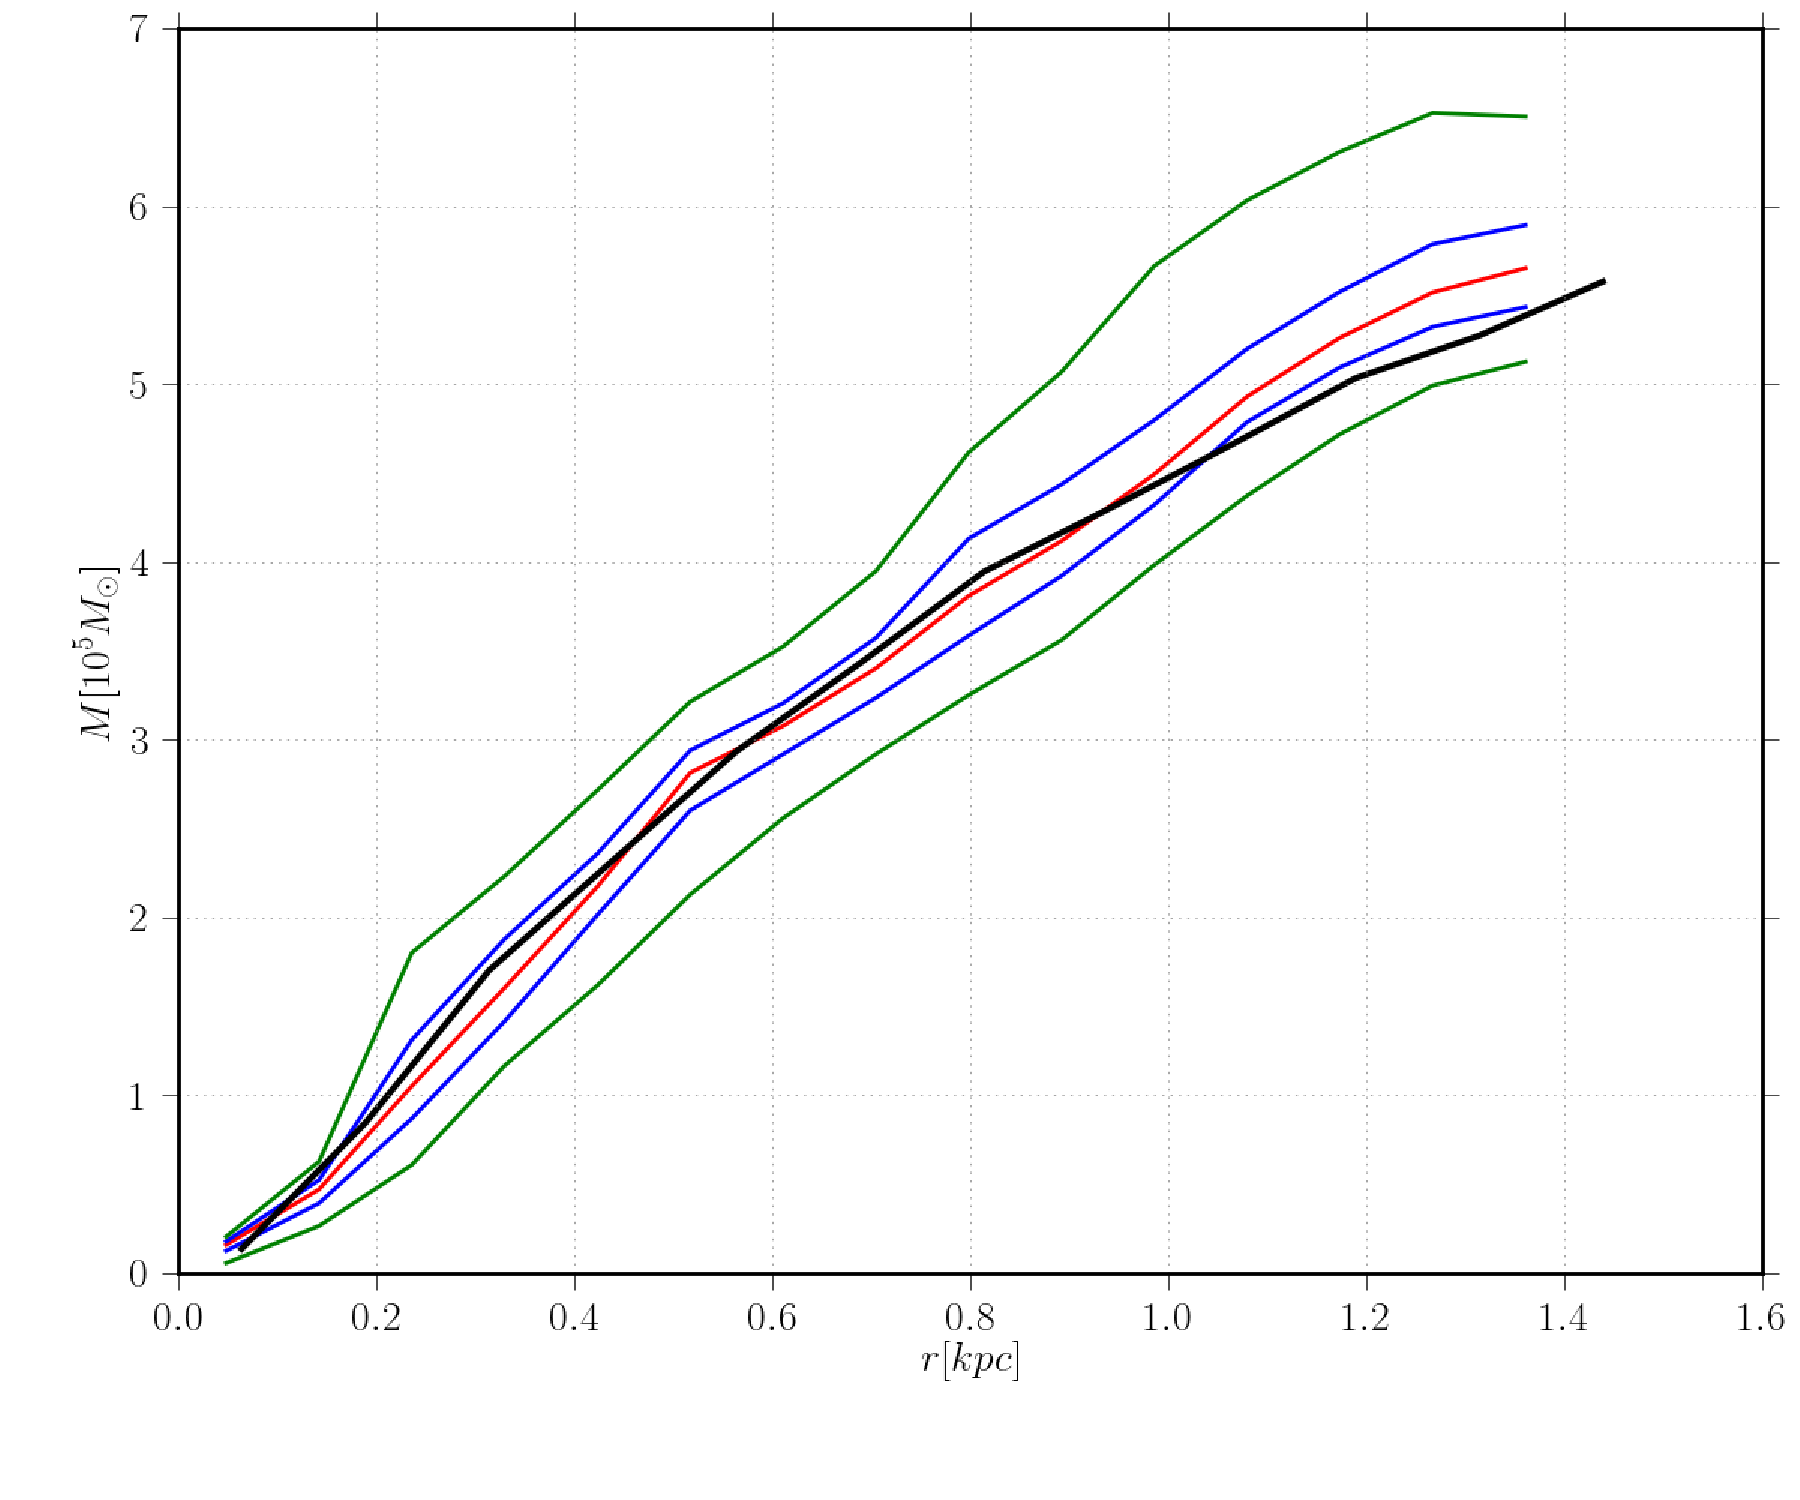
\includegraphics[width=0.3\textwidth]{fig/hernquist1e4.pdf}
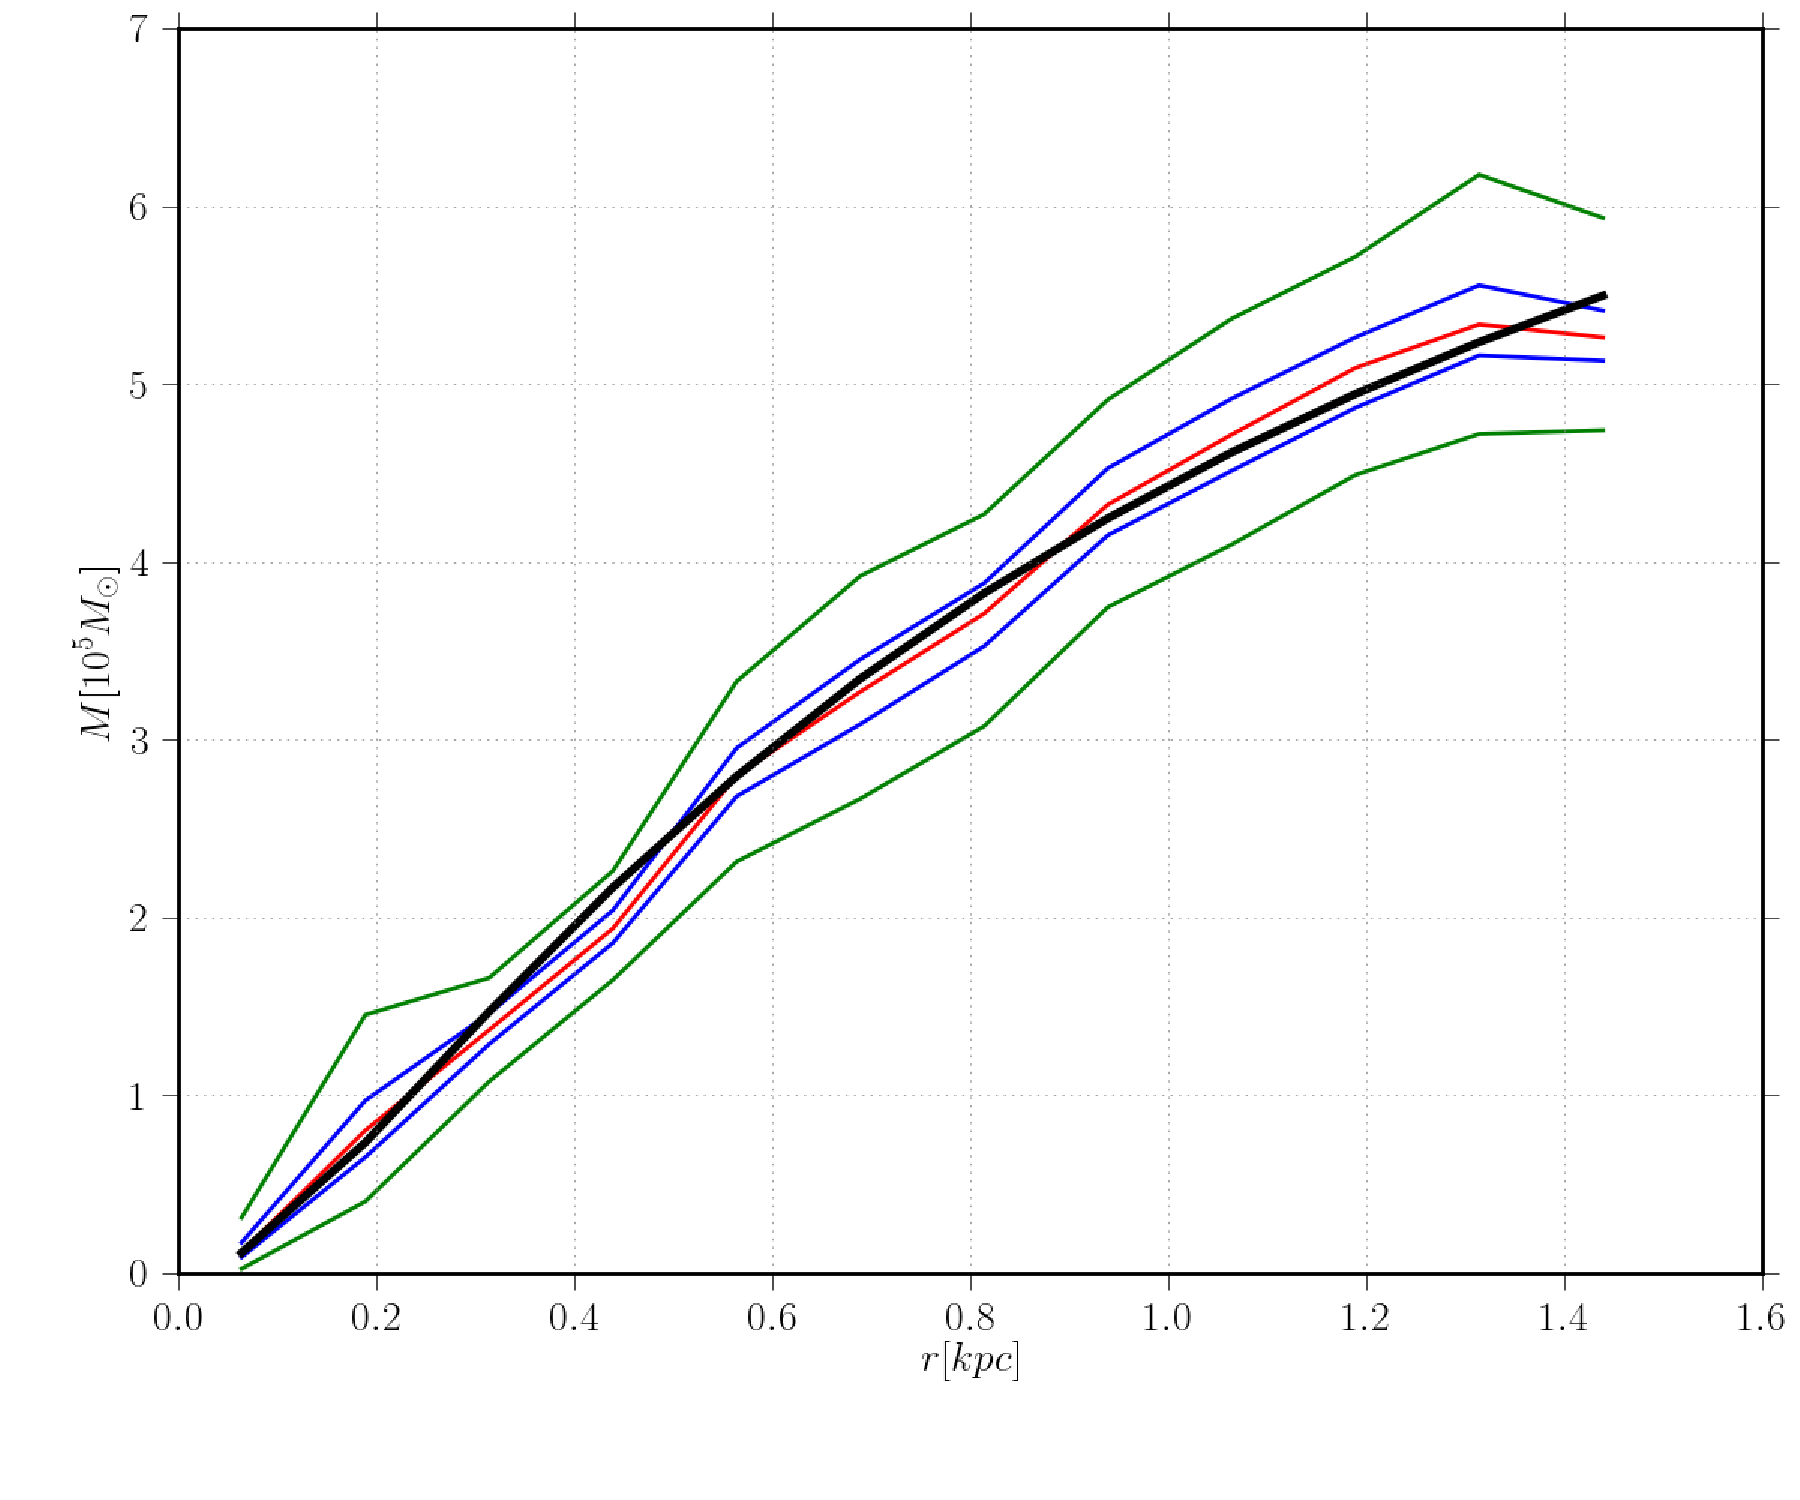
\includegraphics[width=0.3\textwidth]{fig/hernquist2x5e3.pdf}
\caption{Hernquist profile found by MCMC model (red) for $10^3$,
  $10^4$ and two times $5\cdot10^3$ tracer particles. The black curve
  shows the enclosed mass derived from the theoretical model.}
\label{fig:hernquist1e3}
\end{center}
\end{figure*}




\subsection{Effects of turning off priors}
\TODO{turning off $\delta dens>0$}
\TODO{$\beta<0$ prior}



\subsection{Convergence in MCMC}
We check the convergence of the MCMC twofold: first, the range of
density profiles swept after 5k, 50k and to the end of our run is
increased from 5k to 50k, but stays approximately constant for another
16k runs, thus giving us confidence that we found and fully explored
the valid regions of phase space in density. See fig. \ref{fig:convergencedens}.

\begin{figure*}
\begin{center}
\hspace{-7mm}
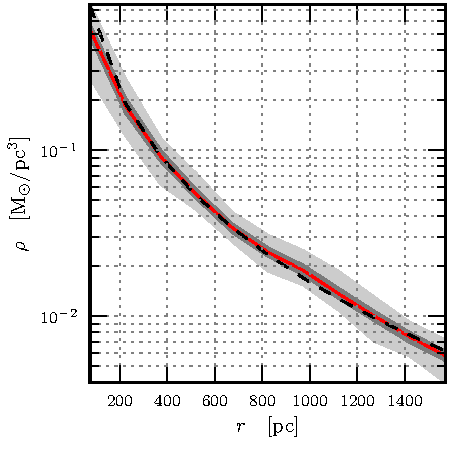
\includegraphics[width=0.3\textwidth]{fig/20130718132442_case_2_10000_0_cprior_nulog_denslog_mslope_rprior_5kits_profdens.pdf}
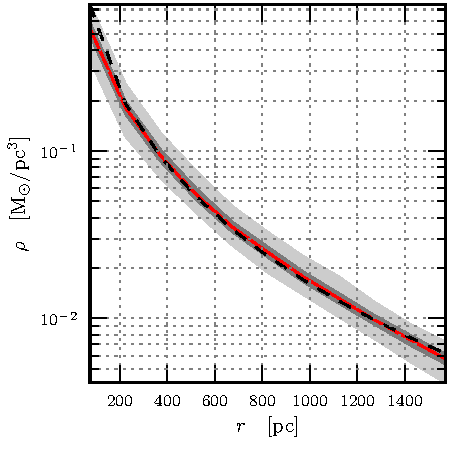
\includegraphics[width=0.3\textwidth]{fig/20130718132442_case_2_10000_0_cprior_nulog_denslog_mslope_rprior_50kits_profdens.pdf}
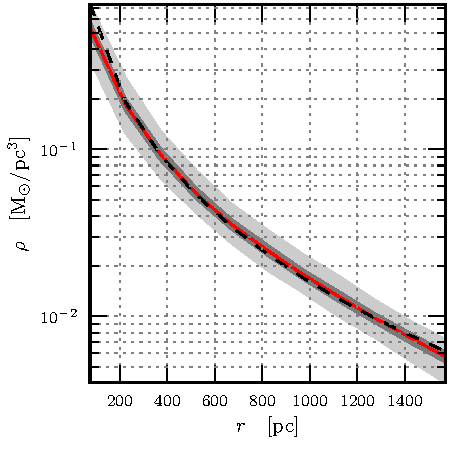
\includegraphics[width=0.3\textwidth]{fig/20130718132442_case_2_10000_0_cprior_nulog_denslog_mslope_rprior_67kits_profdens.pdf}
\caption{Convergence of the density profile after (5k,50k,67k) iterations (left to right).}
\label{fig:convergencedens}
\end{center}
\end{figure*}

Second, the range of $\delta_i$, the only other unrestricted
parameters, show a similar behaviour, as shown in
\ref{fig:convergencedelta1} for $\delta_1$, with analogous
$\delta_2$. \TODO{Not all the parameter space is sampled, and this is
  a major cause of worry: any profile found in the first iterations in
  the init phase will be stuck there, if $\delta$ cannot sample a big
  subset of $]-\infty,1]$. We will rerun thge cusp for proper $10^6$
  iterations, with higher stepsize for delta!}

\begin{figure*}
\begin{center}
\hspace{-7mm}
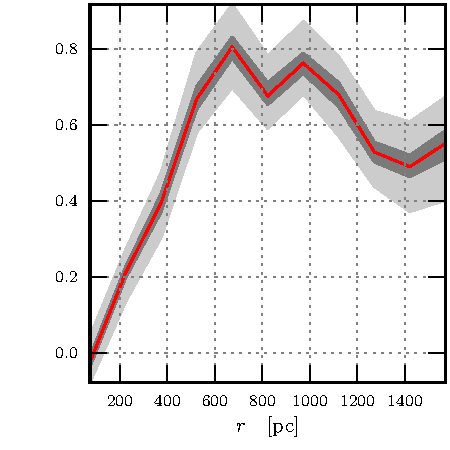
\includegraphics[width=0.3\textwidth]{fig/20130718132442_case_2_10000_0_cprior_nulog_denslog_mslope_rprior_5kit_profdelta1.pdf}
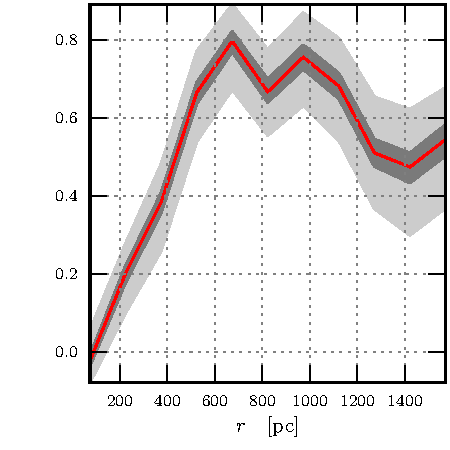
\includegraphics[width=0.3\textwidth]{fig/20130718132442_case_2_10000_0_cprior_nulog_denslog_mslope_rprior_50kit_profdelta1.pdf}
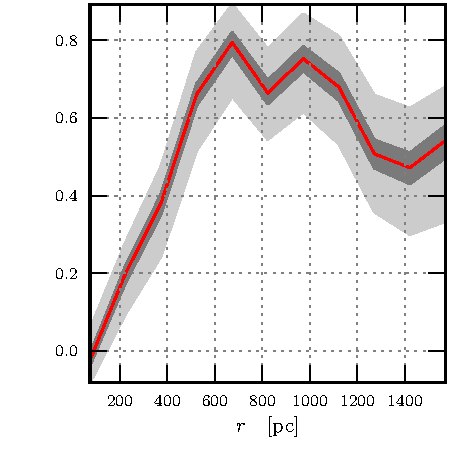
\includegraphics[width=0.3\textwidth]{fig/20130718132442_case_2_10000_0_cprior_nulog_denslog_mslope_rprior_67kit_profdelta1.pdf}
\caption{Convergence of $\delta_1$ after (5k,50k,67k) iterations (left to right).}
\label{fig:convergencedelta1}
\end{center}
\end{figure*}





\subsection{Convergence in Mass Models}
\TODO{constant number of particles per bin}



\subsection{Splitting by metallicities}\label{sec:metals}

Observations of the abundances of metals and chemical species in the
stellar atmospheres show that the ensemble of stars in a dwarf galaxy
or globular cluster can be split into populations.

The first approach by \cite{WalkerPenarrubia2012} showed that if the
population of e.g. Fornax is split into two populations, and each of
their half-light radius and mass are determined, restrictions on the
overall potential can be drawn. Using this approach, they prefer a
cored DM profile for Fornax.

In our test suite there are dwarf galaxies with different scale radii
and small differences in the mean of the metallicity for the two
populations of stars. In order to reproduce the underlying populations
we use an inset MCMC with assumptions that

\begin{enumerate}
\item Foreground stars are younger than most of the dSph member
  stars. Therefore, they show a high metallicity and can be removed
  from the dataset with a single cut in metallicity;
\item the remaining stellar components are divided into two
  populations;
\item the fraction of stars in population 1 is sampled in a uniform
  way in the range $[0.2,0.8]$;
\item both populations show a normal distribution in metallicity with
  the same width;
\item the initial values of the means are set to half and twice the
  mean metallicity, to allow for a reasonable difference between the
  means. This difference is then subsequently sampled assuming a
  normal distribution;
\item 40000 iterations for burn-in and 10000 iterations for subsequent
  parameter estimates are used, with a thinning by factor 10 to reduce
  correlations between subsequent models. This procedure converges in
  all tested cases.
\end{enumerate}

To test whether the assignment into populations is a valid one, we
want to check whether the population is in equilibrium with the
overall potential.

\begin{figure*}
\begin{center}
\hspace{-7mm}
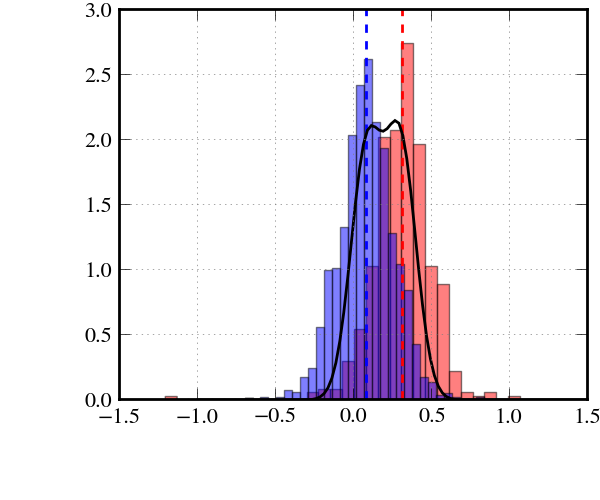
\includegraphics[width=0.5\textwidth]{fig/pymcmetals.png}
\caption{Distribution function of two populations (filled histograms) and the reproduced overall distribution.}
\label{fig:pops}
\end{center}
\end{figure*}

The routine then assigns each particle to one of the two populations,
based on its Mg metallicity. $75\pm4\%$ of all stars are assigned to
the correct underlying distribution. This in turn changes the
half-light radius by $110$pc and $-62$pc for initial 390 pc, 730 pc
half light radii. These changes are rather high, but the two
populations still show distinct half-light radii.


We explicitly assume two populations of stellar tracers in dwarf
galaxies, each with Gaussian distributions in metallicity with means
$\mu_1,\mu_2$. Without requiring a minimum distance $\delta
\mu=\mu_2-\mu_1$ between them, a representation with $\mu_1 \approx
\mu_2$ can be found. This model shows a higher $\chi^2$ than other
models and is thus disfavoured, but cannot be rejected from a
Kolmogorov-Smirnov test on a $p<0.05$ basis.

Here we show the influence of setting a prior minimal
$\delta\mu_{\min}$ on the goodness of fit, and the allowed range of
$\delta \mu$. We work on the metallicity distribution of one of the
mock dwarfs with cusped density profiles described earlier on, setting

\begin{equation}
\mu_1\in[-1.0,2.0];\quad \delta \mu \in [ \delta\mu_{\min}, 5.0];\quad 
\end{equation}

with $\delta\mu_{\min}$ varying from $0.0$ to $0.4$. We let the MCMC
run for a) 10k iterations with 8k burn-in/discarded models; b) 50k
iterations with 40k burn-in. From the accepted models, we compute the
mean Gaussian distributions and compare the corresponding overall
bimodal distribution to the actual metallicity distribution from the
data with a 2 component Kolmogorov-Smirnov test, and take the
two-tailed statistics $p$ from 30 drawings. If the $p>0.05$, then we
cannot reject the hypothesis that the distributions of the two samples
are the same.

Results for varying the minimal distance between the two Gaussians
between $0.0$ and $0.4$ are shown in fig \ref{fig:kit}.

\begin{figure*}
\begin{center}
\hspace{-7mm}
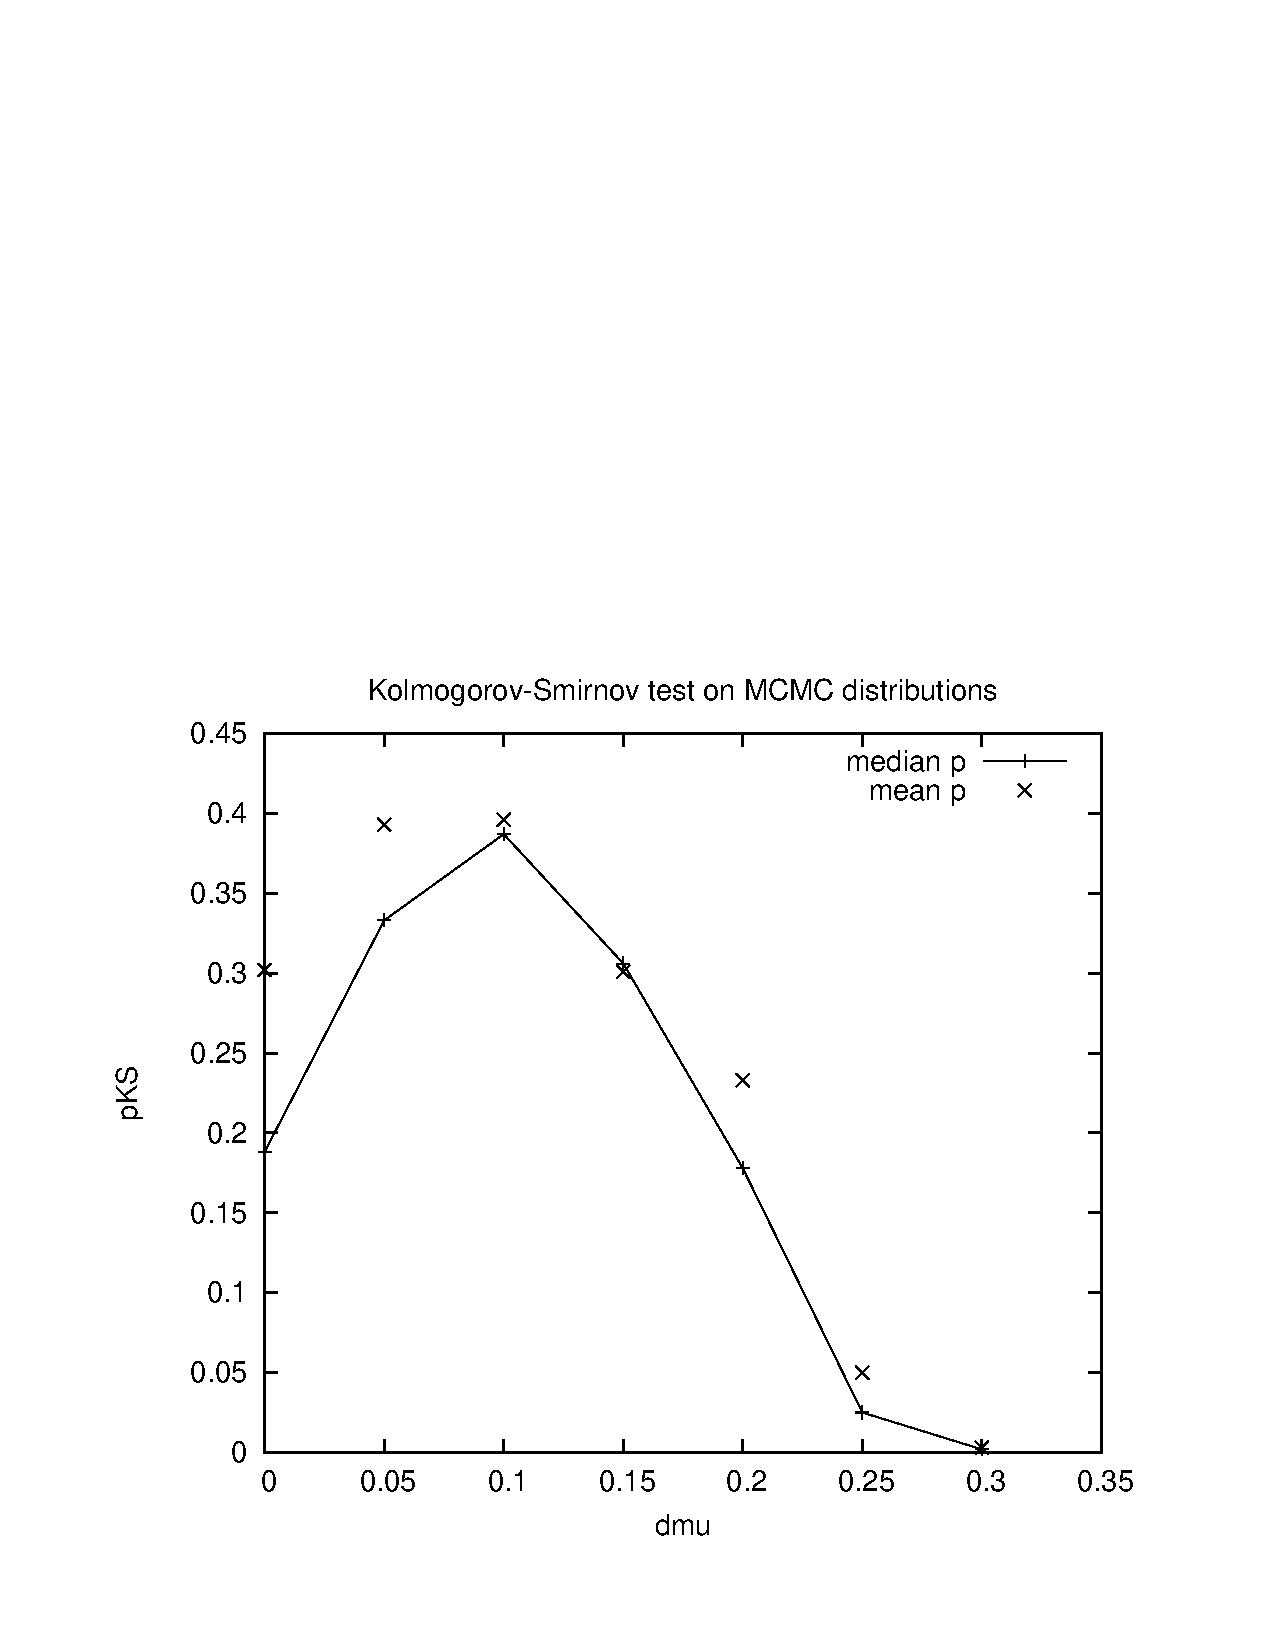
\includegraphics[width=0.5\textwidth]{fig/10kit.pdf}
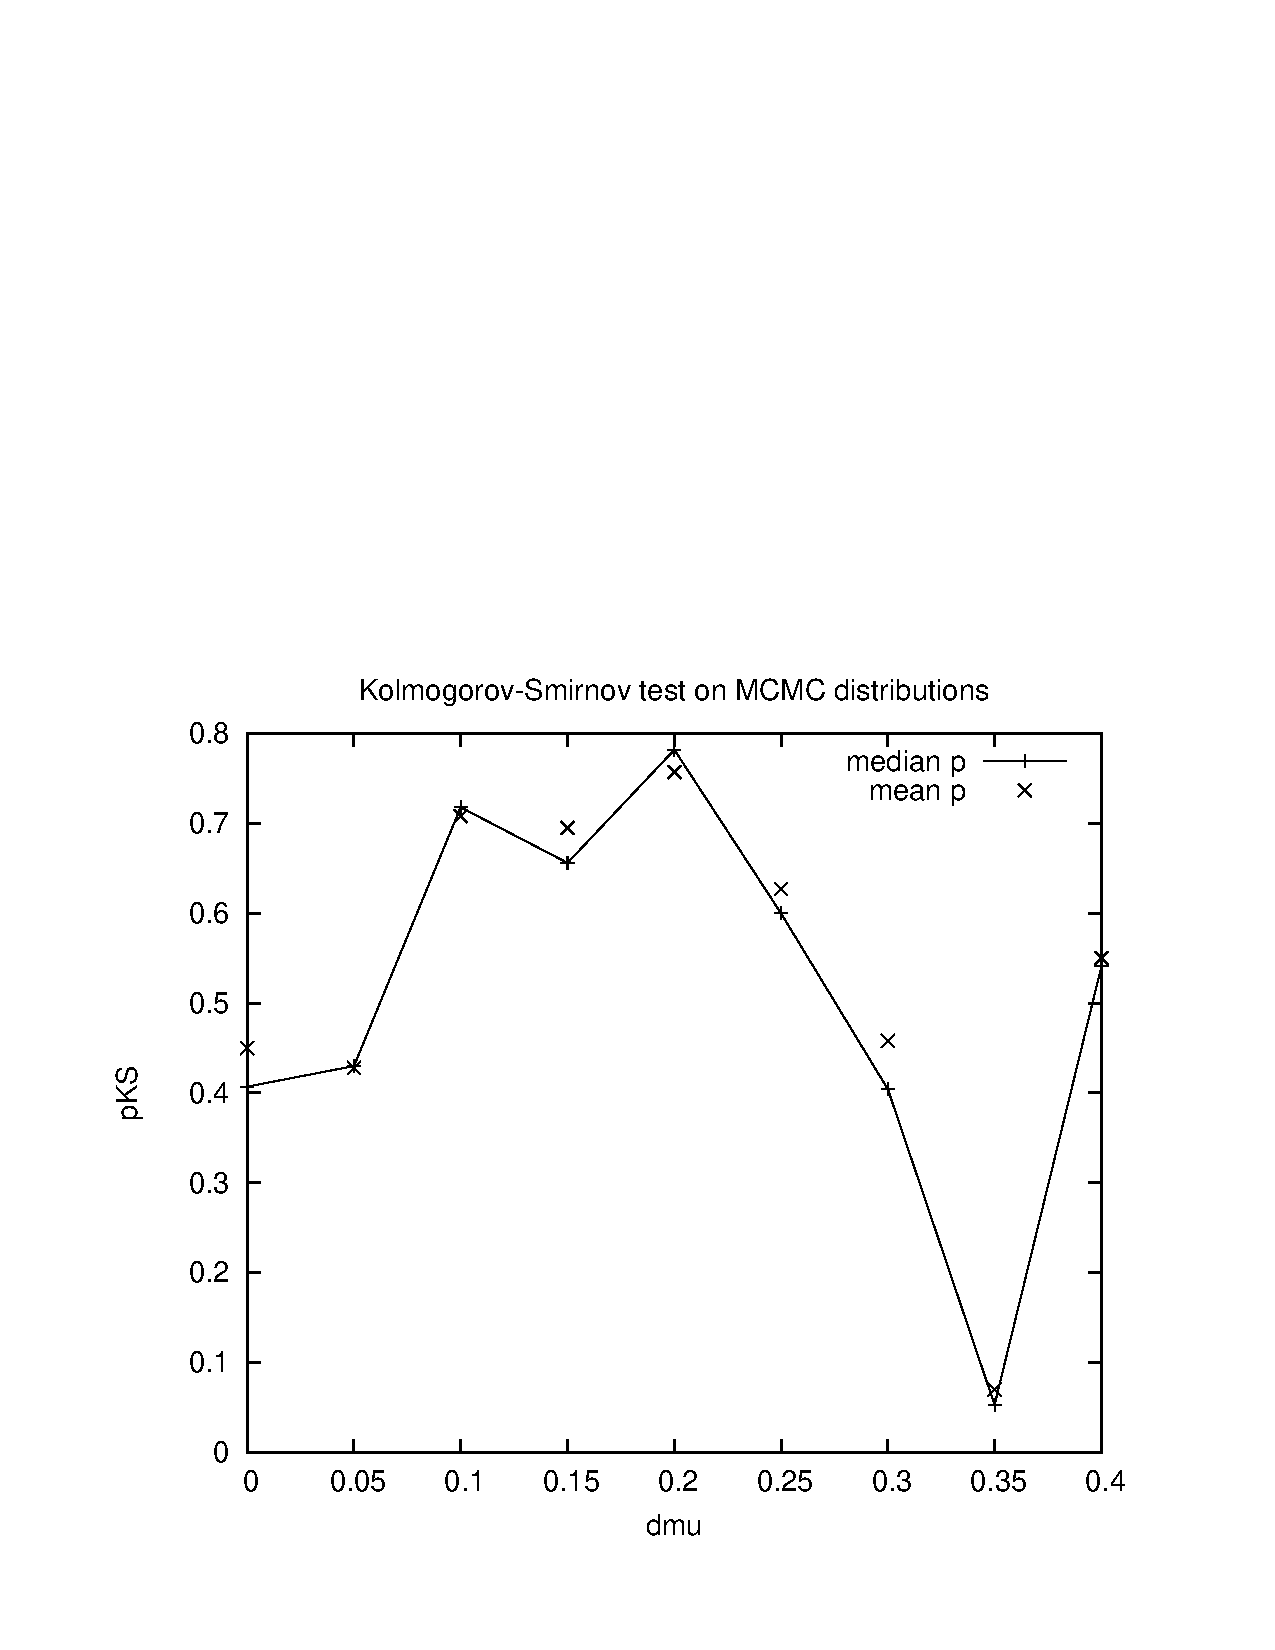
\includegraphics[width=0.5\textwidth]{fig/50kit.pdf}
\caption{Kolmogorov-Smirnov test for correspondance between models
  with $\delta\mu>\delta\mu_{\min}$ as described in the text.}
\label{fig:kit}
\end{center}
\end{figure*}


All models with $p>0.05$ give a reasonable fit, with a maximum for 10k
iterations at around $\delta \mu = 0.1$. Models with $\delta \mu>0.2$
give no good fit anymore after 10k iterations.

The goodness of fit is enhanced if we take more iterations, so in the
plot for 50k iterations, there is a maximum $p=0.79$ compared to
$p=0.4$ from 10k iterations only. The whole curve is shifted to higher
$\delta \mu$ values. The models with $\delta \mu>0.3$ are
rejected. The restriction of $\delta \mu>0.4$ (last point to the
right) is well-fitting again, but this is due to the fact that the
fraction of particles for population 2 was found to be smaller than 10
percent, thus mainly fitting the metallicity distribution with one
Gaussian only, plus some skewing from an almost negligible stellar
component. Although this model cannot be rejected, it lies above the
rejected models at $\delta\mu_{\min}=0.4$. Furthermore, it does not
yield a second component with a scale length distinctly different from
the main component, rendering the additional gain from two components
obsolete. Thus, we will restrict the MCMC search of the population
fraction to the range $f\in[0.3,0.7]$.






\subsection{Effect of Wrong Assignment of Populations}
